
%% bare_jrnl.tex
%% V1.4b
%% 2015/08/26
%% by Michael Shell
%% see http://www.michaelshell.org/
%% for current contact information.
%%
%% This is a skeleton file demonstrating the use of IEEEtran.cls
%% (requires IEEEtran.cls version 1.8b or later) with an IEEE
%% journal paper.
%%
%% Support sites:
%% http://www.michaelshell.org/tex/ieeetran/
%% http://www.ctan.org/pkg/ieeetran
%% and
%% http://www.ieee.org/

%%*************************************************************************
%% Legal Notice:
%% This code is offered as-is without any warranty either expressed or
%% implied; without even the implied warranty of MERCHANTABILITY or
%% FITNESS FOR A PARTICULAR PURPOSE! 
%% User assumes all risk.
%% In no event shall the IEEE or any contributor to this code be liable for
%% any damages or losses, including, but not limited to, incidental,
%% consequential, or any other damages, resulting from the use or misuse
%% of any information contained here.
%%
%% All comments are the opinions of their respective authors and are not
%% necessarily endorsed by the IEEE.
%%
%% This work is distributed under the LaTeX Project Public License (LPPL)
%% ( http://www.latex-project.org/ ) version 1.3, and may be freely used,
%% distributed and modified. A copy of the LPPL, version 1.3, is included
%% in the base LaTeX documentation of all distributions of LaTeX released
%% 2003/12/01 or later.
%% Retain all contribution notices and credits.
%% ** Modified files should be clearly indicated as such, including  **
%% ** renaming them and changing author support contact information. **
%%*************************************************************************


% *** Authors should verify (and, if needed, correct) their LaTeX system  ***
% *** with the testflow diagnostic prior to trusting their LaTeX platform ***
% *** with production work. The IEEE's font choices and paper sizes can   ***
% *** trigger bugs that do not appear when using other class files.       ***                          ***
% The testflow support page is at:
% http://www.michaelshell.org/tex/testflow/



\documentclass[journal]{IEEEtran}
%
% If IEEEtran.cls has not been installed into the LaTeX system files,
% manually specify the path to it like:
% \documentclass[journal]{../sty/IEEEtran}

\usepackage{float}
\usepackage[section]{placeins} % \FloatBarrier, it avoids floating of tables and



% Some very useful LaTeX packages include:
% (uncomment the ones you want to load)


% *** MISC UTILITY PACKAGES ***
%
%\usepackage{ifpdf}
% Heiko Oberdiek's ifpdf.sty is very useful if you need conditional
% compilation based on whether the output is pdf or dvi.
% usage:
% \ifpdf
%   % pdf code
% \else
%   % dvi code
% \fi
% The latest version of ifpdf.sty can be obtained from:
% http://www.ctan.org/pkg/ifpdf
% Also, note that IEEEtran.cls V1.7 and later provides a builtin
% \ifCLASSINFOpdf conditional that works the same way.
% When switching from latex to pdflatex and vice-versa, the compiler may
% have to be run twice to clear warning/error messages.






% *** CITATION PACKAGES ***
%
\usepackage{cite}
% cite.sty was written by Donald Arseneau
% V1.6 and later of IEEEtran pre-defines the format of the cite.sty package
% \cite{} output to follow that of the IEEE. Loading the cite package will
% result in citation numbers being automatically sorted and properly
% "compressed/ranged". e.g., [1], [9], [2], [7], [5], [6] without using
% cite.sty will become [1], [2], [5]--[7], [9] using cite.sty. cite.sty's
% \cite will automatically add leading space, if needed. Use cite.sty's
% noadjust option (cite.sty V3.8 and later) if you want to turn this off
% such as if a citation ever needs to be enclosed in parenthesis.
% cite.sty is already installed on most LaTeX systems. Be sure and use
% version 5.0 (2009-03-20) and later if using hyperref.sty.
% The latest version can be obtained at:
% http://www.ctan.org/pkg/cite
% The documentation is contained in the cite.sty file itself.


\usepackage{graphicx}
\graphicspath{{Images/}} %% Path to find Image Files



% *** GRAPHICS RELATED PACKAGES ***
%
\ifCLASSINFOpdf
  % \usepackage[pdftex]{graphicx}
  % declare the path(s) where your graphic files are
  % \graphicspath{{../pdf/}{../jpeg/}}
  % and their extensions so you won't have to specify these with
  % every instance of \includegraphics
  % \DeclareGraphicsExtensions{.pdf,.jpeg,.png}
\else
  % or other class option (dvipsone, dvipdf, if not using dvips). graphicx
  % will default to the driver specified in the system graphics.cfg if no
  % driver is specified.
  % \usepackage[dvips]{graphicx}
  % declare the path(s) where your graphic files are
  % \graphicspath{{../eps/}}
  % and their extensions so you won't have to specify these with
  % every instance of \includegraphics
  % \DeclareGraphicsExtensions{.eps}
\fi
% graphicx was written by David Carlisle and Sebastian Rahtz. It is
% required if you want graphics, photos, etc. graphicx.sty is already
% installed on most LaTeX systems. The latest version and documentation
% can be obtained at: 
% http://www.ctan.org/pkg/graphicx
% Another good source of documentation is "Using Imported Graphics in
% LaTeX2e" by Keith Reckdahl which can be found at:
% http://www.ctan.org/pkg/epslatex
%
% latex, and pdflatex in dvi mode, support graphics in encapsulated
% postscript (.eps) format. pdflatex in pdf mode supports graphics
% in .pdf, .jpeg, .png and .mps (metapost) formats. Users should ensure
% that all non-photo figures use a vector format (.eps, .pdf, .mps) and
% not a bitmapped formats (.jpeg, .png). The IEEE frowns on bitmapped formats
% which can result in "jaggedy"/blurry rendering of lines and letters as
% well as large increases in file sizes.
%
% You can find documentation about the pdfTeX application at:
% http://www.tug.org/applications/pdftex





% *** MATH PACKAGES ***
%
\usepackage{amsmath}
% A popular package from the American Mathematical Society that provides
% many useful and powerful commands for dealing with mathematics.
%
% Note that the amsmath package sets \interdisplaylinepenalty to 10000
% thus preventing page breaks from occurring within multiline equations. Use:
%\interdisplaylinepenalty=2500
% after loading amsmath to restore such page breaks as IEEEtran.cls normally
% does. amsmath.sty is already installed on most LaTeX systems. The latest
% version and documentation can be obtained at:
% http://www.ctan.org/pkg/amsmath


% limits underneath
\DeclareMathOperator*{\argmax}{arg\,max} % Jan Hlavacek



% *** SPECIALIZED LIST PACKAGES ***
%
%\usepackage{algorithmic}
% algorithmic.sty was written by Peter Williams and Rogerio Brito.
% This package provides an algorithmic environment fo describing algorithms.
% You can use the algorithmic environment in-text or within a figure
% environment to provide for a floating algorithm. Do NOT use the algorithm
% floating environment provided by algorithm.sty (by the same authors) or
% algorithm2e.sty (by Christophe Fiorio) as the IEEE does not use dedicated
% algorithm float types and packages that provide these will not provide
% correct IEEE style captions. The latest version and documentation of
% algorithmic.sty can be obtained at:
% http://www.ctan.org/pkg/algorithms
% Also of interest may be the (relatively newer and more customizable)
% algorithmicx.sty package by Szasz Janos:
% http://www.ctan.org/pkg/algorithmicx




% *** ALIGNMENT PACKAGES ***
%
\usepackage{array}
% Frank Mittelbach's and David Carlisle's array.sty patches and improves
% the standard LaTeX2e array and tabular environments to provide better
% appearance and additional user controls. As the default LaTeX2e table
% generation code is lacking to the point of almost being broken with
% respect to the quality of the end results, all users are strongly
% advised to use an enhanced (at the very least that provided by array.sty)
% set of table tools. array.sty is already installed on most systems. The
% latest version and documentation can be obtained at:
% http://www.ctan.org/pkg/array


% IEEEtran contains the IEEEeqnarray family of commands that can be used to
% generate multiline equations as well as matrices, tables, etc., of high
% quality.




% *** SUBFIGURE PACKAGES ***
%\ifCLASSOPTIONcompsoc
%  \usepackage[caption=false,font=normalsize,labelfont=sf,textfont=sf]{subfig}
%\else
%  \usepackage[caption=false,font=footnotesize]{subfig}
%\fi
% subfig.sty, written by Steven Douglas Cochran, is the modern replacement
% for subfigure.sty, the latter of which is no longer maintained and is
% incompatible with some LaTeX packages including fixltx2e. However,
% subfig.sty requires and automatically loads Axel Sommerfeldt's caption.sty
% which will override IEEEtran.cls' handling of captions and this will result
% in non-IEEE style figure/table captions. To prevent this problem, be sure
% and invoke subfig.sty's "caption=false" package option (available since
% subfig.sty version 1.3, 2005/06/28) as this is will preserve IEEEtran.cls
% handling of captions.
% Note that the Computer Society format requires a larger sans serif font
% than the serif footnote size font used in traditional IEEE formatting
% and thus the need to invoke different subfig.sty package options depending
% on whether compsoc mode has been enabled.
%
% The latest version and documentation of subfig.sty can be obtained at:
% http://www.ctan.org/pkg/subfig




% *** FLOAT PACKAGES ***
%
\usepackage{fixltx2e}
% fixltx2e, the successor to the earlier fix2col.sty, was written by
% Frank Mittelbach and David Carlisle. This package corrects a few problems
% in the LaTeX2e kernel, the most notable of which is that in current
% LaTeX2e releases, the ordering of single and double column floats is not
% guaranteed to be preserved. Thus, an unpatched LaTeX2e can allow a
% single column figure to be placed prior to an earlier double column
% figure.
% Be aware that LaTeX2e kernels dated 2015 and later have fixltx2e.sty's
% corrections already built into the system in which case a warning will
% be issued if an attempt is made to load fixltx2e.sty as it is no longer
% needed.
% The latest version and documentation can be found at:
% http://www.ctan.org/pkg/fixltx2e


%\usepackage{stfloats}
% stfloats.sty was written by Sigitas Tolusis. This package gives LaTeX2e
% the ability to do double column floats at the bottom of the page as well
% as the top. (e.g., "\begin{figure*}[!b]" is not normally possible in
% LaTeX2e). It also provides a command:
%\fnbelowfloat
% to enable the placement of footnotes below bottom floats (the standard
% LaTeX2e kernel puts them above bottom floats). This is an invasive package
% which rewrites many portions of the LaTeX2e float routines. It may not work
% with other packages that modify the LaTeX2e float routines. The latest
% version and documentation can be obtained at:
% http://www.ctan.org/pkg/stfloats
% Do not use the stfloats baselinefloat ability as the IEEE does not allow
% \baselineskip to stretch. Authors submitting work to the IEEE should note
% that the IEEE rarely uses double column equations and that authors should try
% to avoid such use. Do not be tempted to use the cuted.sty or midfloat.sty
% packages (also by Sigitas Tolusis) as the IEEE does not format its papers in
% such ways.
% Do not attempt to use stfloats with fixltx2e as they are incompatible.
% Instead, use Morten Hogholm'a dblfloatfix which combines the features
% of both fixltx2e and stfloats:
%
% \usepackage{dblfloatfix}
% The latest version can be found at:
% http://www.ctan.org/pkg/dblfloatfix




%\ifCLASSOPTIONcaptionsoff
%  \usepackage[nomarkers]{endfloat}
% \let\MYoriglatexcaption\caption
% \renewcommand{\caption}[2][\relax]{\MYoriglatexcaption[#2]{#2}}
%\fi
% endfloat.sty was written by James Darrell McCauley, Jeff Goldberg and 
% Axel Sommerfeldt. This package may be useful when used in conjunction with 
% IEEEtran.cls'  captionsoff option. Some IEEE journals/societies require that
% submissions have lists of figures/tables at the end of the paper and that
% figures/tables without any captions are placed on a page by themselves at
% the end of the document. If needed, the draftcls IEEEtran class option or
% \CLASSINPUTbaselinestretch interface can be used to increase the line
% spacing as well. Be sure and use the nomarkers option of endfloat to
% prevent endfloat from "marking" where the figures would have been placed
% in the text. The two hack lines of code above are a slight modification of
% that suggested by in the endfloat docs (section 8.4.1) to ensure that
% the full captions always appear in the list of figures/tables - even if
% the user used the short optional argument of \caption[]{}.
% IEEE papers do not typically make use of \caption[]'s optional argument,
% so this should not be an issue. A similar trick can be used to disable
% captions of packages such as subfig.sty that lack options to turn off
% the subcaptions:
% For subfig.sty:
% \let\MYorigsubfloat\subfloat
% \renewcommand{\subfloat}[2][\relax]{\MYorigsubfloat[]{#2}}
% However, the above trick will not work if both optional arguments of
% the \subfloat command are used. Furthermore, there needs to be a
% description of each subfigure *somewhere* and endfloat does not add
% subfigure captions to its list of figures. Thus, the best approach is to
% avoid the use of subfigure captions (many IEEE journals avoid them anyway)
% and instead reference/explain all the subfigures within the main caption.
% The latest version of endfloat.sty and its documentation can obtained at:
% http://www.ctan.org/pkg/endfloat
%
% The IEEEtran \ifCLASSOPTIONcaptionsoff conditional can also be used
% later in the document, say, to conditionally put the References on a 
% page by themselves.




% *** PDF, URL AND HYPERLINK PACKAGES ***
%
%\usepackage{url}
% url.sty was written by Donald Arseneau. It provides better support for
% handling and breaking URLs. url.sty is already installed on most LaTeX
% systems. The latest version and documentation can be obtained at:
% http://www.ctan.org/pkg/url
% Basically, \url{my_url_here}.




% *** Do not adjust lengths that control margins, column widths, etc. ***
% *** Do not use packages that alter fonts (such as pslatex).         ***
% There should be no need to do such things with IEEEtran.cls V1.6 and later.
% (Unless specifically asked to do so by the journal or conference you plan
% to submit to, of course. )


% correct bad hyphenation here
\hyphenation{op-tical net-works semi-conduc-tor}


\begin{document}
%
% paper title
% Titles are generally capitalized except for words such as a, an, and, as,
% at, but, by, for, in, nor, of, on, or, the, to and up, which are usually
% not capitalized unless they are the first or last word of the title.
% Linebreaks \\ can be used within to get better formatting as desired.
% Do not put math or special symbols in the title.
\title{ARMA Time Series Modeling for Solar PV Generation Forecasting}
%
%
% author names and IEEE memberships
% note positions of commas and nonbreaking spaces ( ~ ) LaTeX will not break
% a structure at a ~ so this keeps an author's name from being broken across
% two lines.
% use \thanks{} to gain access to the first footnote area
% a separate \thanks must be used for each paragraph as LaTeX2e's \thanks
% was not built to handle multiple paragraphs
%

\author{Ninad Gaikwad and Karthikeya Devaprasad}

% note the % following the last \IEEEmembership and also \thanks - 
% these prevent an unwanted space from occurring between the last author name
% and the end of the author line. i.e., if you had this:
% 
% \author{....lastname \thanks{...} \thanks{...} }
%                     ^------------^------------^----Do not want these spaces!
%
% a space would be appended to the last name and could cause every name on that
% line to be shifted left slightly. This is one of those "LaTeX things". For
% instance, "\textbf{A} \textbf{B}" will typeset as "A B" not "AB". To get
% "AB" then you have to do: "\textbf{A}\textbf{B}"
% \thanks is no different in this regard, so shield the last } of each \thanks
% that ends a line with a % and do not let a space in before the next \thanks.
% Spaces after \IEEEmembership other than the last one are OK (and needed) as
% you are supposed to have spaces between the names. For what it is worth,
% this is a minor point as most people would not even notice if the said evil
% space somehow managed to creep in.



% The paper headers
\markboth{Optimal Estimation and Kalman Filtering Project Proposal, November~2018}%
{Shell \MakeLowercase{\textit{et al.}}: Bare Demo of IEEEtran.cls for IEEE Journals}
% The only time the second header will appear is for the odd numbered pages
% after the title page when using the twoside option.
% 
% *** Note that you probably will NOT want to include the author's ***
% *** name in the headers of peer review papers.                   ***
% You can use \ifCLASSOPTIONpeerreview for conditional compilation here if
% you desire.




% If you want to put a publisher's ID mark on the page you can do it like
% this:
%\IEEEpubid{0000--0000/00\$00.00~\copyright~2015 IEEE}
% Remember, if you use this you must call \IEEEpubidadjcol in the second
% column for its text to clear the IEEEpubid mark.



% use for special paper notices
%\IEEEspecialpapernotice{(Invited Paper)}




% make the title area
\maketitle

% As a general rule, do not put math, special symbols or citations
% in the abstract or keywords.
\begin{abstract}
There has been a recent push to integrate renewable sources of energy into the power grid, with Solar PV being one of the most promising among them. Among other things, effective integration involves the ability to predict generation so that other sources can be curtailed or increased accordingly to meet the power demand. Time series modeling is the preferred technique due to the complexity of the factors. This project will explore the effect of various factors like training data size and resolution, and time series model order on the prediction accuracy. We will also be implementing custom programs to estimate the model parameters, make predictions and evaluate these models.
\end{abstract}

% Note that keywords are not normally used for peerreview papers.
\begin{IEEEkeywords}
ARMA, Time Series, Solar PV, Forecasting
\end{IEEEkeywords}






% For peer review papers, you can put extra information on the cover
% page as needed:
% \ifCLASSOPTIONpeerreview
% \begin{center} \bfseries EDICS Category: 3-BBND \end{center}
% \fi
%
% For peerreview papers, this IEEEtran command inserts a page break and
% creates the second title. It will be ignored for other modes.
\IEEEpeerreviewmaketitle



\section{Introduction}


\subsection{Solar PV}
Due to the irreversible effects of Global Warming, there is a worldwide initiative to integrate renewable sources of energy into the power grid. Solar Photo-Voltaic (PV) generation is the most prominent among these that is being explored and is promising due to the lower upfront costs involved, ease of installation and adoption, and the passive nature of generation with minimal human oversight. However, one of the major drawbacks associated with it is the restriction of power generation to hours of daylight. The demands of the grid that are not met by solar will have to be balanced out by other conventional and renewable sources. Therefore, the effective integration of solar will require the ability to predict the amount and duration of solar PV power generation, and effectively using other sources to match the excess demand.

\subsection{Time Series Forecasting}

A time-series is a set of data points that is spaced at equal intervals of time. In time-series forecasting, we use time-series data to create system models which use past time instants as input and generate predictions of future time instants as outputs. This model is then used to make predictions about future instants.
\\
Time series forecasting is a very important technique that is used in a wide array of fields like Economics, Statistics, Weather-Forecasting and Signal Processing. It is generally adopted when the system is too complex to be represented as a mathematical model of various other inputs resulting in an output. This may be because of the complex relationships between the various inputs affecting the output, or the lack of input data that is spaced at the same time intervals as the output training data. \cite{gagniuc2017markov}
\\
In these cases, a time series model is used, wherein the output prediction of a random variable at any time-instant is a linear result of the random variable at past time instants. The output will not depend on other inputs to the system, unlike other conventional system models.


\subsection{Time Series Forecasting for Solar PV Generation Forecasting}

The power generated by a Solar PV cell is dependent on various factors like Incident Solar Radiation Intensity, the ambient temperature as well as the meteorological conditions. All these factors are strongly correlated, which makes it very difficult to characterize the power generated as a function of these parameters. \cite{zhou2007novel} Therefore, we choose to use a time-series model where the solar power generation is the only variable considered and the power generation at any time instant is a function of the power generated at past instants. \cite{huang2012solar}

\subsection{Auto-Regressive Moving Average (ARMA) Model}

“A stationary process is a stochastic process whose unconditional joint probability distribution does not change when shifted in time. It’s parameters such as mean and variance do not change over time. Such a process can be described using an ARMA model, consisting of two polynomials. One of these is for the autoregression (AR) and the second is for the moving average (MA). The AR part involves regressing the variable on its own lagged values. The MA part involves modeling the error term as a linear combination of error terms occurring contemporaneously and at various times in the past. The model is usually referred to as the ARMA (p,q) model where p is the order of the AR part and q is the order of the MA part.”
\\
“ARMA models can be estimated using the Box-Jenkins method.” \cite{box2015time} \cite{baillie2017maximum} \cite{sandgren2012moving}
\\
%By studying the past Solar Generation data, we can see that the process is weakly stationary with AR and MA components having a seasonality of 24 hours. Therefore, we have initially tried using an AR(4) model to make the forecasting and see how well it compares with the actual measured data. This model is also being used to create the Least Squares and Max Likelihood estimation functions for the model parameters. However, the model requires further changes to improve accuracy and we may need to incorporate a Moving Average component.


\section{Problem Statement}

Using ARMA time series modeling to create prediction models for forecasting power generated by Solar Photovoltaic (PV) arrays using the Diamond Solar data. Developing and evaluating ARMA prediction models for various time scales of the Diamond Solar Data. Finally, evaluating the effect of different estimation techniques used to estimate the parameters of the ARMA models on the performance of prediction models.


\section{Aims and Objectives}

The aims and objectives are as follows;



\begin{itemize}
  \item Transforming the given Diamond Solar Data (5min Resolution) to different time scales – 15 min, 60 min, 120 min, 180 min, Daily and Monthly resolution data.
  \item Using MATLAB’s Econometrics Toolbox to develop ARMA models for the above-mentioned time scales and predict solar power generation.

  \item Developing ARMA estimation models based on Least Squares (LS) and Maximum Likelihood Estimation (MLE) to develop solar power generation models at different time scales using the appropriate model orders obtained previously from the Econometrics Toolbox.
  \item For intra-day time scales training data of one week and two weeks will be used respectively for training the above-mentioned models and a forecast of one week into the future will be generated. 
  \item Comparing the accuracy of the generated forecasts from the MATLAB’s Econometrics Toolbox and the developed ARMA Estimation models, different developed ARMA estimation models, different amount of training data and different time scales will be done.
  \item Evaluating the effect of different ARMA parameter estimation models on the forecast accuracy.
  \item Evaluating the effect of amount of training data on the forecast accuracy.
  \item Evaluating the effectiveness of ARMA prediction on different time scales
  
   
\end{itemize}




\section{Methods}

The method comprises of three main parts:  Data Pre-Processing, Development of ARMA models using MATLAB's Econometrics Toolbox and Development of ARMA Parameter Estimation techniques based on Least Squares and Maximum Loglikelihood Estimation. The schematic of the method is illustrated in Fig. \ref{fig1}.

\begin{figure}[htpb]
\centering
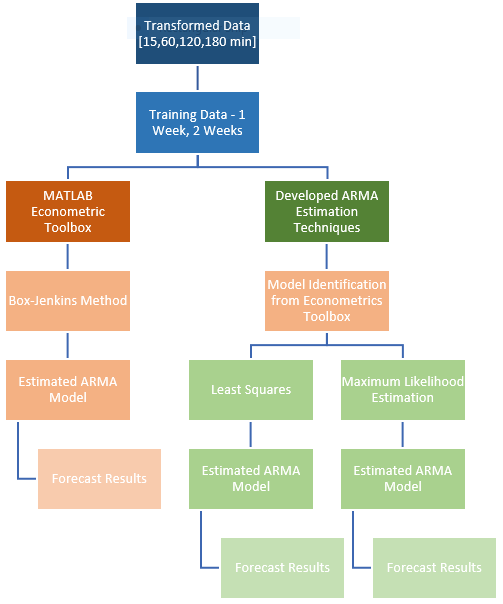
\includegraphics[scale=0.4]{ObjectivesSchematic.png}
\caption{ARMA Model Development Schematic}
\label{fig1} %% to refer use, \ref{}
\end{figure}

\subsection{Data Pre-Processing}



The data file Diamond\_Solar\_data.csv consists of three different time series at 5 minutes resolution corresponding to Diamond300, Diamond304 and Diamond306 contiguously arranged in a single column. This file is processed to give individual files corresponding to Diamond300, Diamond304 and Diamond306 at different time resolutions of 5 min, 15 min, 60 min, 2 hours (120 min), 3 hours (180 min), daily and monthly. The schematic for data pre-processing is illustrated in Fig. \ref{fig2}. The transformed data for 15 minute and one hour intervals are plotted against the original five minute data in Fig. \ref{fig3}. We can observe that averaging the data over an entire hour removes the large fluctuations seen with the five-minute and fifteen-minute data. While this will provide better prediction models, it will also result in a loss of resolution.

\begin{figure}[htpb]
\centering
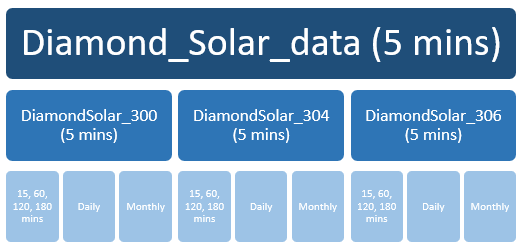
\includegraphics[scale=0.65]{DataTransformationSchematic.png}
\caption{Data Pre-Processing Schematic}
\label{fig2} %% to refer use, \ref{}
\end{figure}

\begin{figure}[htpb]
	\centering
	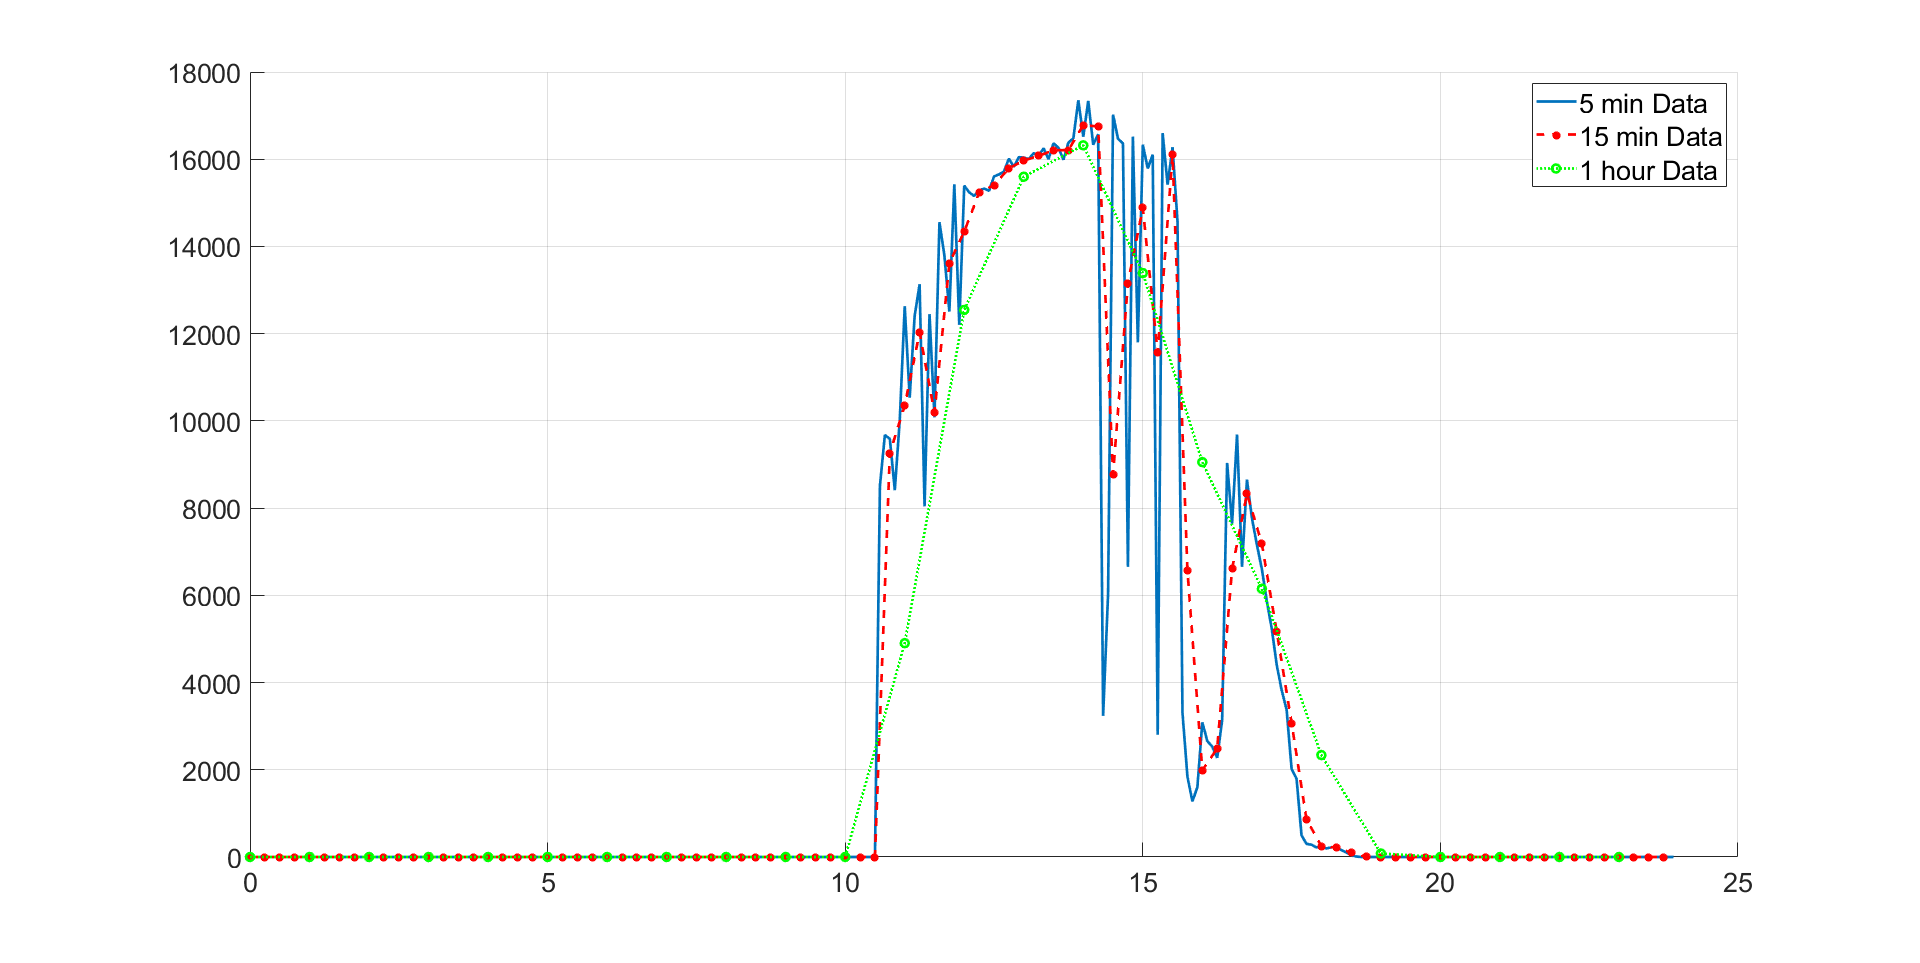
\includegraphics[scale=0.2]{TransformedDataPlot.png}
	\caption{Plot of Transformed Data for 15 min and 1 hour}
	\label{fig3} %% to refer use, \ref{}
\end{figure}



\subsection{ARMA Model Development using MATLAB’s Econometrics Toolbox}

The ARMA model development is done using Box-Jenkins Method \cite{box2015time}, which has the following steps as illustrated in the Fig. \ref{fig4}.


\begin{figure}[htpb]
\centering
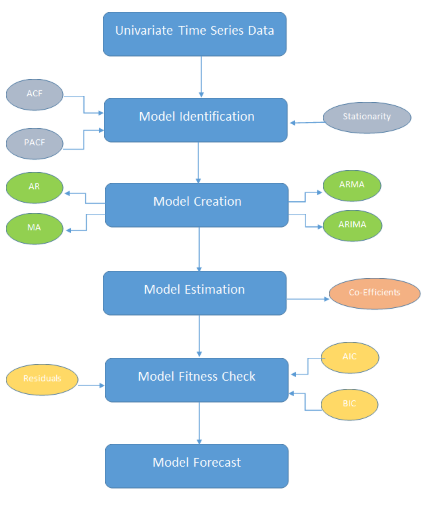
\includegraphics[scale=0.75]{ARMASteps.png}
\caption{ARMA Model Development Schematic}
\label{fig4} %% to refer use, \ref{}
\end{figure}

\begin{enumerate}

  \item \textbf{Model Identification:} The univariate time series is checked for stationarity and if not, stationary it has to be converted into a stationary series by applying differencing. The Auto-Correlation Function (ACF) and the Partial Auto-Correlation Function (PACF) of the stationary univariate time series are checked for determining the order of the AR and MA process generating the series.
  \item \textbf{Model Creation:} On the basis of the Model Identification a number of models around the determined AR and MA orders are created.
  \item \textbf{Model Estimation:} These models are then estimated to give the appropriate coefficients.
  \item \textbf{Model Fitness Check:} The estimated models are then evaluated using Akaike Information Criterion (AIC) and Bayesian Information Criterion (BIC). Lower the AIC and BIC better the model.
  \item \textbf{Model Forecast:} The best model determined from the previous step is used to forecast the series.


\end{enumerate}



\subsection{ARMA Parameter Estimation Techniques}



\subsubsection{Least Squares Estimation Method}

The parameter estimation of an ARMA process using Least Squares is as follows;

\begin{align*}
\widehat{y_{t}} &= a_{1}y_{t-1} + a_{2}y_{t-2} + ... + b_{1}\epsilon_{t-1} + b_{2}\epsilon_{t-2}+ ... + \epsilon_{t}
\end{align*}
Now;
\begin{align*}
\widehat{y_{t}} &= ay + b\epsilon
\end{align*}
Where;
\begin{align*}
a &= [a_{1} \hspace{2mm} a_{2} \hspace{2mm} a_{3} .... ]\\
b &= [b_{1} \hspace{2mm} b_{2} \hspace{2mm} b_{3} .... ]\\
y &= [y_{t-1} \hspace{2mm} y_{t-2} \hspace{2mm} y_{t-3} ...]^{T}\\
\epsilon &= [\epsilon_{t-1} \hspace{2mm} \epsilon_{t-2} \hspace{2mm} \epsilon_{t-3} ...]^{T}
\end{align*}
The Least Squares Estimate for the Parameters is given by;
\begin{align*}
\widehat{\theta}(a,b) &= \operatorname*{arg\,min}_\theta \frac{1}{2} \left[ \left(y_{t}-\widehat{y_{t}} \right)^{2} \right]\\
\end{align*}

\subsubsection{Maximum Likelihood Estimation Method}

The maximum likelihood function for an ARMA process when the error is assumed to be distributed normally is give as follows;

\begin{align*}
\widehat{\theta}(a,b)= \argmax_\theta \frac{1}{\sqrt{2\pi\sigma^{2}}} e^{-\frac{\left(y_{t}-\widehat{y_{t}} \right)^{2}}{2\sigma^{2}}}
\end{align*}

%\begin{align*}
%\widehat{\theta}(a,b)= \argmin_\theta \frac{1}{\sqrt{2\pi\sigma^{2}}} e^{-\frac{\left(y_{t}-\widehat{y_{t} \right)^{2}}}{2\sigma^{2}}}
%\end{align*}

\section{Initial experiments and results}

We have performed some initial experiments on the fifteen minute data and made a few forecasts assuming an AR(4) model with seasonality of 24 hours. The results are as shown in Fig. \ref{fig5} and Fig. \ref{fig6}.

\begin{figure}[htpb]
	\centering
	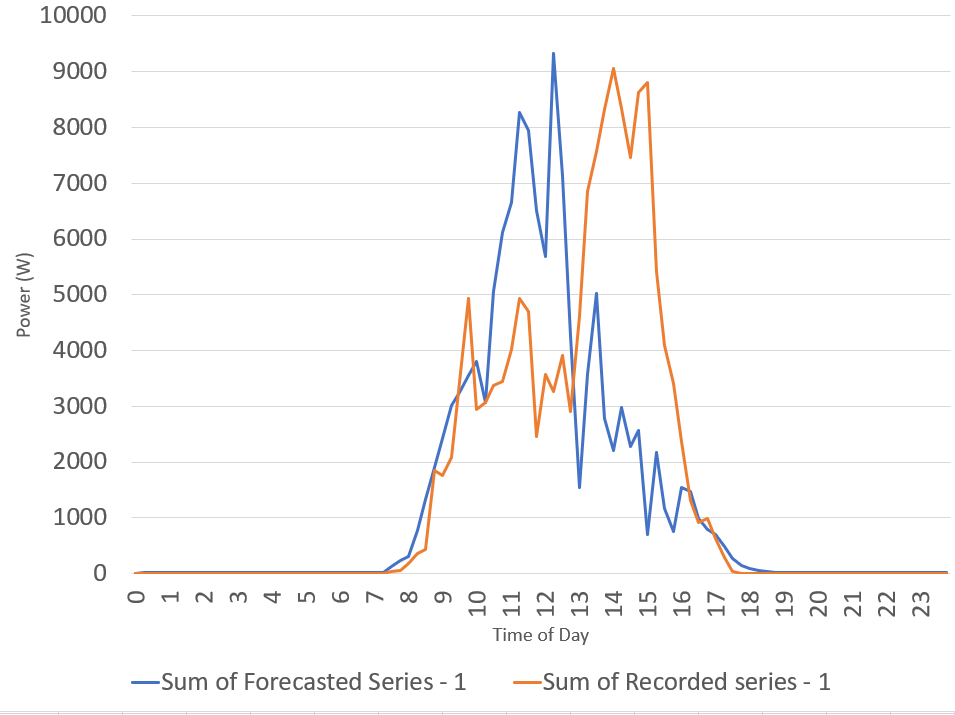
\includegraphics[scale=0.35]{ForecastResultsOneWeek.png}
	\caption{Forecast results for 1st day with a week of training data}
	\label{fig5} %% to refer use, \ref{}
\end{figure}

\begin{figure}[htpb]
	\centering
	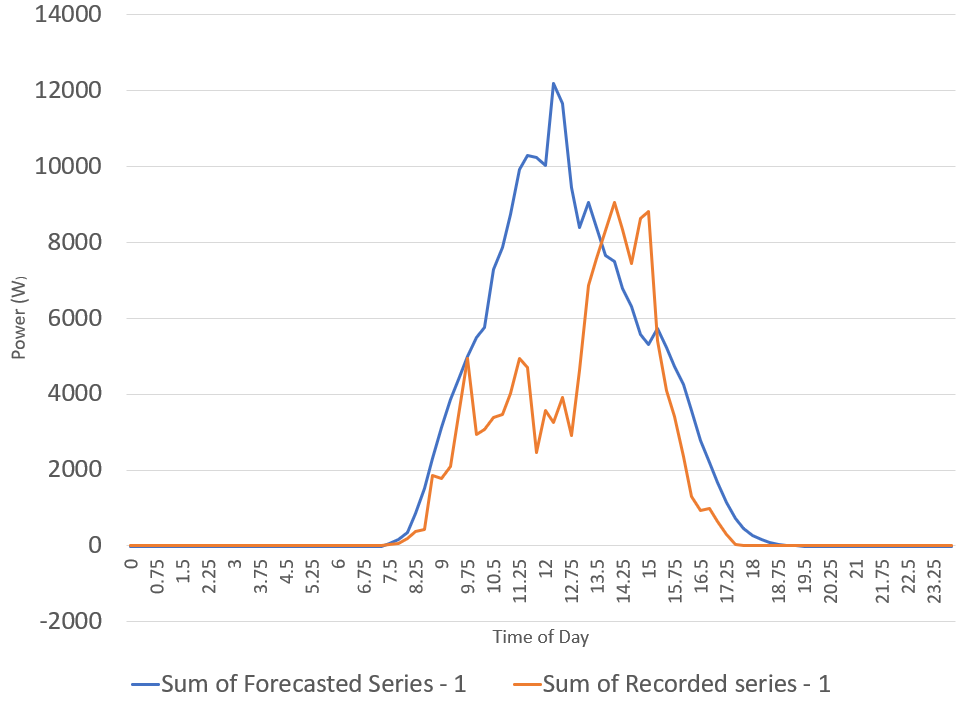
\includegraphics[scale=0.35]{ForecastResultsTwoWeek.png}
	\caption{Forecast results for 1st day with two weeks of training data}
	\label{fig6} %% to refer use, \ref{}
\end{figure}



We can see that the forecast with just one week of training data appears to be closer to the actual observations than the forecast made with two weeks of training data. Therefore, we will need to use an appropriate amount of training data based on the forecast duration we are looking to make, with a week's data sufficient to make a forecast for a single day.
Apart from that, we can see that the day for which the forecast has been made has anomalous recordings due to possible cloud conditions. Therefore, we can see that even a well-tuned ARMA model cannot account for it and will not be able to predict the actual output under such conditions.

\begin{figure}[htpb]
	\centering
	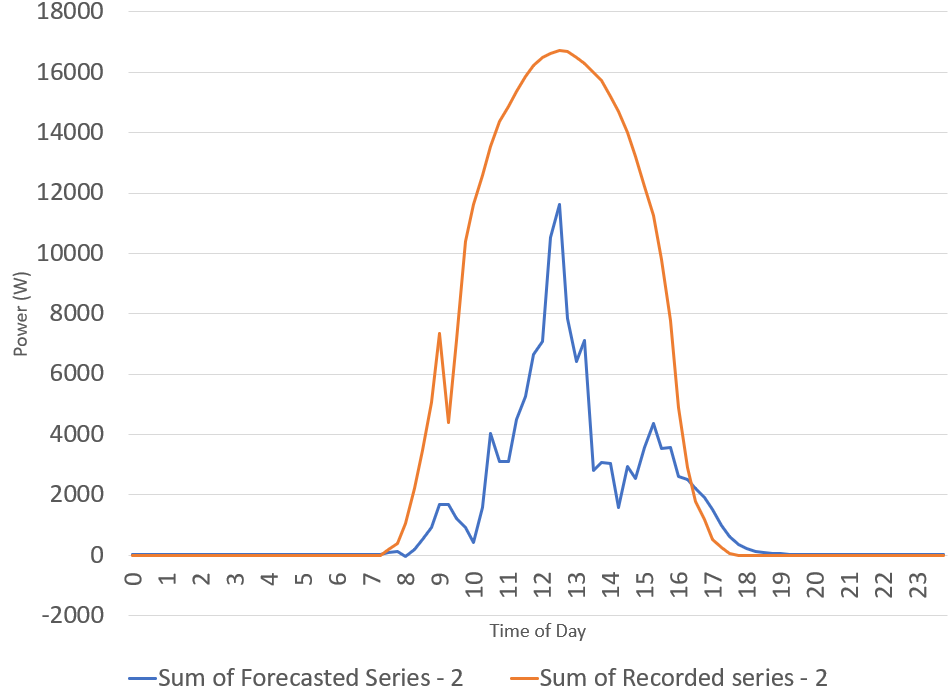
\includegraphics[scale=0.35]{ForecastOneWeekDayTwo.png}
	\caption{Forecast results for 2nd day with a week of training data}
	\label{fig7} %% to refer use, \ref{}
\end{figure}

\begin{figure}[htpb]
	\centering
	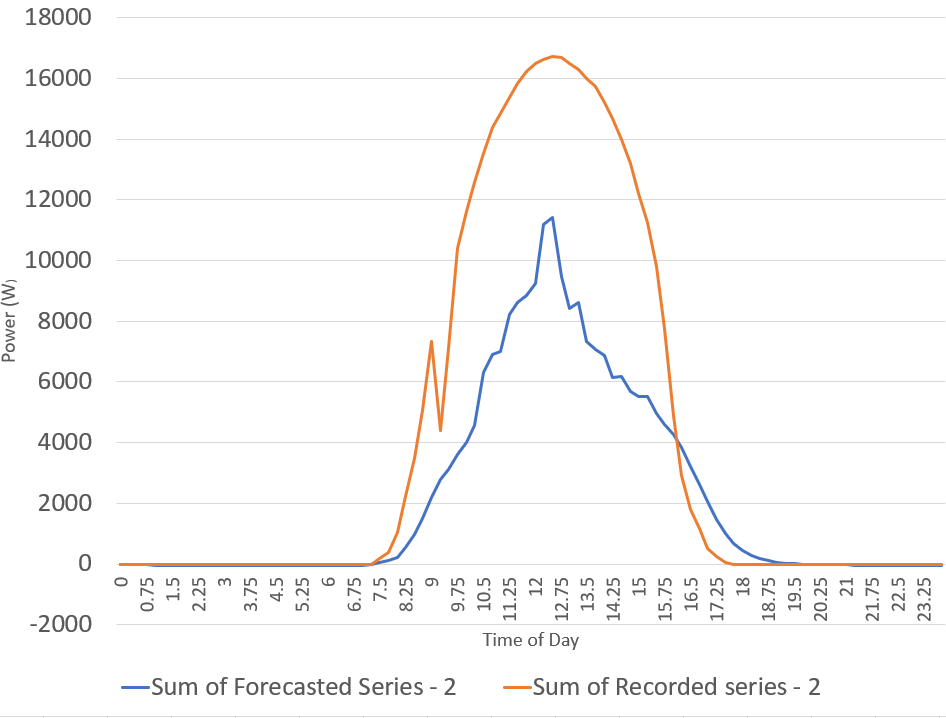
\includegraphics[scale=0.35]{ForecastTwoWeekDayTwo.png}
	\caption{Forecast results for 2nd day with two weeks of training data}
	\label{fig8} %% to refer use, \ref{}
\end{figure}

Fig. \ref{fig7} and Fig. \ref{fig8} show the forecasts for the second day after the training period. We can observe that the accuracy reduces as we make forecasts further away from the training period.

% An example of a floating figure using the graphicx package.
% Note that \label must occur AFTER (or within) \caption.
% For figures, \caption should occur after the \includegraphics.
% Note that IEEEtran v1.7 and later has special internal code that
% is designed to preserve the operation of \label within \caption
% even when the captionsoff option is in effect. However, because
% of issues like this, it may be the safest practice to put all your
% \label just after \caption rather than within \caption{}.
%
% Reminder: the "draftcls" or "draftclsnofoot", not "draft", class
% option should be used if it is desired that the figures are to be
% displayed while in draft mode.
%
%\begin{figure}[!t]
%\centering
%\includegraphics[width=2.5in]{myfigure}
% where an .eps filename suffix will be assumed under latex, 
% and a .pdf suffix will be assumed for pdflatex; or what has been declared
% via \DeclareGraphicsExtensions.
%\caption{Simulation results for the network.}
%\label{fig_sim}
%\end{figure}

% Note that the IEEE typically puts floats only at the top, even when this
% results in a large percentage of a column being occupied by floats.


% An example of a double column floating figure using two subfigures.
% (The subfig.sty package must be loaded for this to work.)
% The subfigure \label commands are set within each subfloat command,
% and the \label for the overall figure must come after \caption.
% \hfil is used as a separator to get equal spacing.
% Watch out that the combined width of all the subfigures on a 
% line do not exceed the text width or a line break will occur.
%
%\begin{figure*}[!t]
%\centering
%\subfloat[Case I]{\includegraphics[width=2.5in]{box}%
%\label{fig_first_case}}
%\hfil
%\subfloat[Case II]{\includegraphics[width=2.5in]{box}%
%\label{fig_second_case}}
%\caption{Simulation results for the network.}
%\label{fig_sim}
%\end{figure*}
%
% Note that often IEEE papers with subfigures do not employ subfigure
% captions (using the optional argument to \subfloat[]), but instead will
% reference/describe all of them (a), (b), etc., within the main caption.
% Be aware that for subfig.sty to generate the (a), (b), etc., subfigure
% labels, the optional argument to \subfloat must be present. If a
% subcaption is not desired, just leave its contents blank,
% e.g., \subfloat[].


% An example of a floating table. Note that, for IEEE style tables, the
% \caption command should come BEFORE the table and, given that table
% captions serve much like titles, are usually capitalized except for words
% such as a, an, and, as, at, but, by, for, in, nor, of, on, or, the, to
% and up, which are usually not capitalized unless they are the first or
% last word of the caption. Table text will default to \footnotesize as
% the IEEE normally uses this smaller font for tables.
% The \label must come after \caption as always.
%
%\begin{table}[!t]
%% increase table row spacing, adjust to taste
%\renewcommand{\arraystretch}{1.3}
% if using array.sty, it might be a good idea to tweak the value of
% \extrarowheight as needed to properly center the text within the cells
%\caption{An Example of a Table}
%\label{table_example}
%\centering
%% Some packages, such as MDW tools, offer better commands for making tables
%% than the plain LaTeX2e tabular which is used here.
%\begin{tabular}{|c||c|}
%\hline
%One & Two\\
%\hline
%Three & Four\\
%\hline
%\end{tabular}
%\end{table}


% Note that the IEEE does not put floats in the very first column
% - or typically anywhere on the first page for that matter. Also,
% in-text middle ("here") positioning is typically not used, but it
% is allowed and encouraged for Computer Society conferences (but
% not Computer Society journals). Most IEEE journals/conferences use
% top floats exclusively. 
% Note that, LaTeX2e, unlike IEEE journals/conferences, places
% footnotes above bottom floats. This can be corrected via the
% \fnbelowfloat command of the stfloats package.




\section{Conclusion}
We have successfully created all the code to preprocess the data and convert it to a series spaced at an appropriate time interval. We have also used this data to create an ARMA model using the in-built MATLAB functions and find estimates for the parameters in the model. The model is able to predict the power generation to a reasonable accuracy level, though further improvements can be made. The final submission will include programs to create a model and estimate its parameters using Least Squares and Max Likelihood estimates.







%The authors would like to thank...


% Can use something like this to put references on a page
% by themselves when using endfloat and the captionsoff option.
\ifCLASSOPTIONcaptionsoff
  \newpage
\fi



% trigger a \newpage just before the given reference
% number - used to balance the columns on the last page
% adjust value as needed - may need to be readjusted if
% the document is modified later
%\IEEEtriggeratref{8}
% The "triggered" command can be changed if desired:
%\IEEEtriggercmd{\enlargethispage{-5in}}

% references section

% can use a bibliography generated by BibTeX as a .bbl file
% BibTeX documentation can be easily obtained at:
% http://mirror.ctan.org/biblio/bibtex/contrib/doc/
% The IEEEtran BibTeX style support page is at:
% http://www.michaelshell.org/tex/ieeetran/bibtex/
%\bibliographystyle{IEEEtran}
% argument is your BibTeX string definitions and bibliography database(s)
%\bibliography{citations.bib}
%
% <OR> manually copy in the resultant .bbl file
% set second argument of \begin to the number of references
% (used to reserve space for the reference number labels box)
%\begin{thebibliography}{1}

\bibliographystyle{IEEEtran}
\bibliography{citations}
%\end{thebibliography}

% biography section
% 
% If you have an EPS/PDF photo (graphicx package needed) extra braces are
% needed around the contents of the optional argument to biography to prevent
% the LaTeX parser from getting confused when it sees the complicated
% \includegraphics command within an optional argument. (You could create
% your own custom macro containing the \includegraphics command to make things
% simpler here.)
%\begin{IEEEbiography}[{\includegraphics[width=1in,height=1.25in,clip,keepaspectratio]{mshell}}]{Michael Shell}
% or if you just want to reserve a space for a photo:



% insert where needed to balance the two columns on the last page with
% biographies
%\newpage


% You can push biographies down or up by placing
% a \vfill before or after them. The appropriate
% use of \vfill depends on what kind of text is
% on the last page and whether or not the columns
% are being equalized.

%\vfill

% Can be used to pull up biographies so that the bottom of the last one
% is flush with the other column.
%\enlargethispage{-5in}



% that's all folks
\end{document}

